%!TEX root = ../article.tex

%%%%%%%%%%%%%%%%%%%%%%%%%%%%%%%%%%%%%%%%%%%%%%%%%%%%%%%%%%%%%%%%%%%%%%%%%%%%%%%
%%%%%%%%%%%%%%%%%%%%%%%%%%%%%%%%%%%%%%%%%%%%%%%%%%%%%%%%%%%%%%%%%%%%%%%%%%%%%%%
\section{Experiments}
\label{sec:experiments}
%%%%%%%%%%%%%%%%%%%%%%%%%%%%%%%%%%%%%%%%%%%%%%%%%%%%%%%%%%%%%%%%%%%%%%%%%%%%%%%
%%%%%%%%%%%%%%%%%%%%%%%%%%%%%%%%%%%%%%%%%%%%%%%%%%%%%%%%%%%%%%%%%%%%%%%%%%%%%%%


% Also an image that is in the \texttt{prebuiltimages/} directory can also be loaded the same way:

% \begin{figure}[h] % h stands for here, ! forces even more...
% 	\centering
% 	
\includegraphics[width=0.2\textwidth]{umontpellier_logo}
% 	\caption{Illustration of a prebuiltimage available.}
% 	\label{fig:umontpellier_logo}
% \end{figure}


% For displaying side by side some images one should consider the package \lstinline+subcaptions+, that can be loaded with the \LaTeX command:

% \begin{lstlisting}[language=tex]
% \usepackage{subcaption}
% \end{lstlisting}


% \begin{figure}[t] % t stands for top (up!)
%     \centering
%     \begin{subfigure}[b]{0.33\textwidth}
%     	\centering
%         
\includegraphics[width=0.2\textwidth]{umontpellier_logo}%
%         \caption{First example}
%         \label{subfig:pythagore}
%     \end{subfigure}
%     \begin{subfigure}[b]{0.56\textwidth}
%     	\centering
%         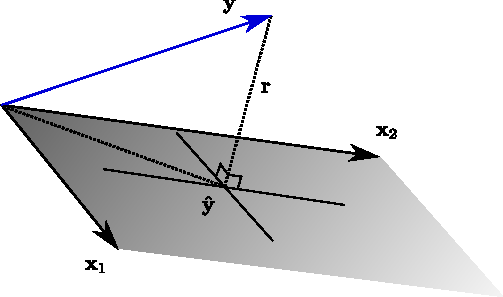
\includegraphics[width=0.5\textwidth]{residu_orth}%
%         \caption{Second example}
%         \label{subfig:logo}
%     \end{subfigure}
%     \caption{Exemples of side by side images}
%     \label{fig:double_example}
% \end{figure}

\subsection{MSE, SURE and F1 score baseline}

\begin{figure}[h]
    \centering
    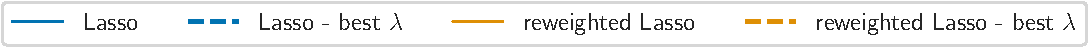
\includegraphics[scale=0.5]{metric_comparison/sure_mse_f1_comparison_legend}
    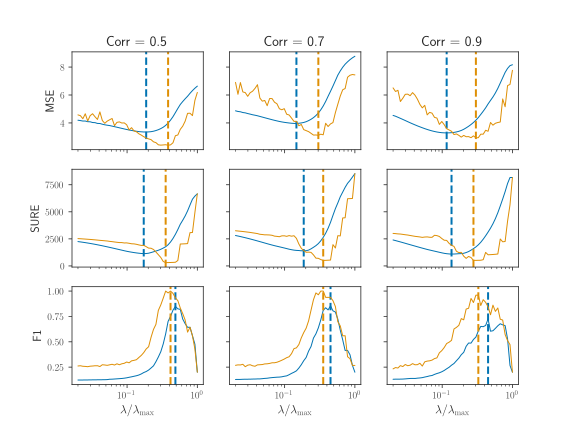
\includegraphics[scale=0.5]{metric_comparison/sure_mse_f1_comparison}
    \caption{SURE, MSE, F1 comparison, \textcolor{blue}{TODO explain more in legend}}
    \label{fig:sure_mse_f1_comparison}
\end{figure}

\subsection{Left Auditory experiments}

\begin{figure}
    \centering
    \begin{subfigure}{6cm}
        \centering 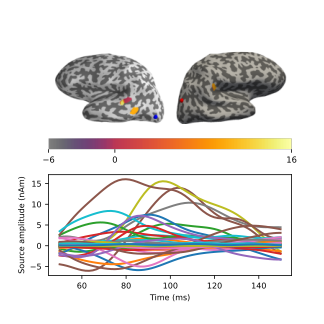
\includegraphics[scale=0.6]{blobs/blob-left_auditory-lasso-cv}
        \caption{Lasso - Held-out MSE}
    \end{subfigure}
    \begin{subfigure}{6cm}
        \centering 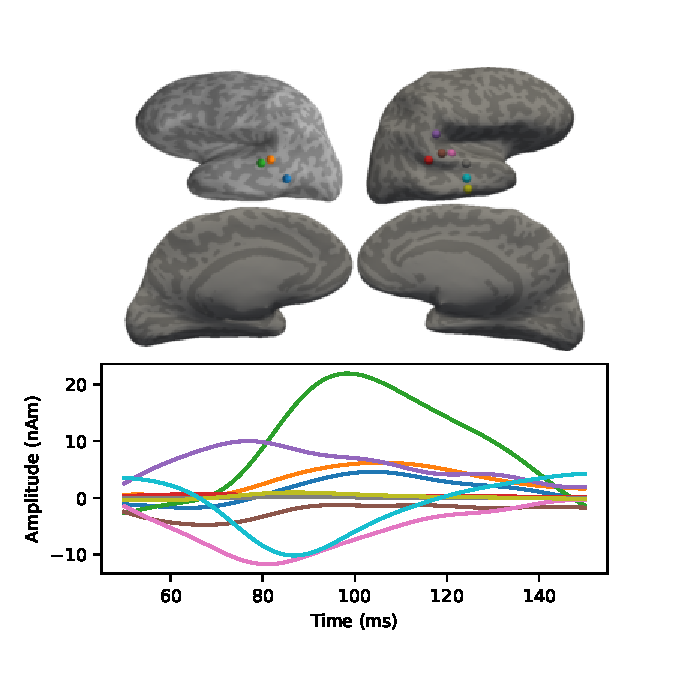
\includegraphics[scale=0.6]{blobs/blob-left_auditory-lasso-sure}
        \caption{Lasso - SURE}
    \end{subfigure}

    \begin{subfigure}{6cm}
        \centering 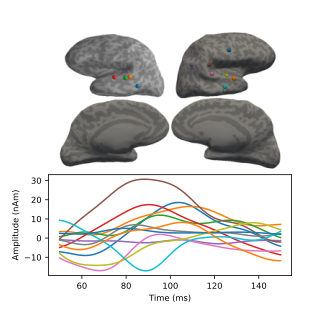
\includegraphics[scale=0.6]{blobs/blob-left_auditory-adaptive-cv}
        \caption{Reweighted - Held-out MSE}
    \end{subfigure}
    \begin{subfigure}{6cm}
        \centering 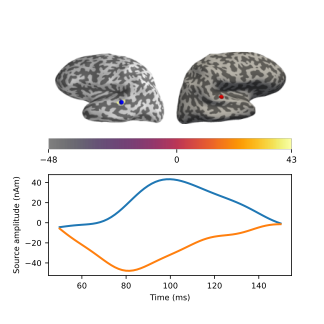
\includegraphics[scale=0.6]{blobs/blob-left_auditory-adaptive-sure}
        \caption{Reweighted - SURE}
    \end{subfigure}
\end{figure}


\subsection{Right Auditory experiments}

\begin{figure}
    \centering
    \begin{subfigure}{6cm}
        \centering 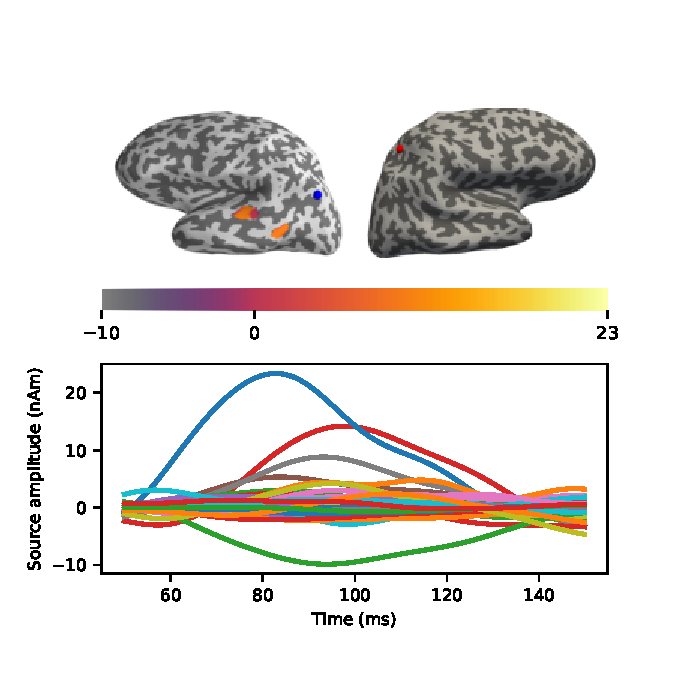
\includegraphics[scale=0.6]{blobs/blob-right_auditory-lasso-cv}
        \caption{Lasso - Held-out MSE}
    \end{subfigure}
    \begin{subfigure}{6cm}
        \centering 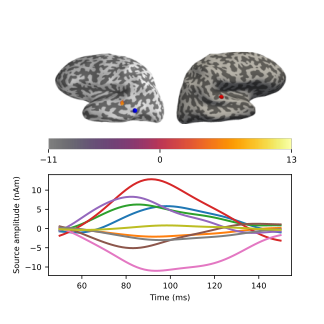
\includegraphics[scale=0.6]{blobs/blob-right_auditory-lasso-sure}
        \caption{Lasso - SURE}
    \end{subfigure}

    \begin{subfigure}{6cm}
        \centering 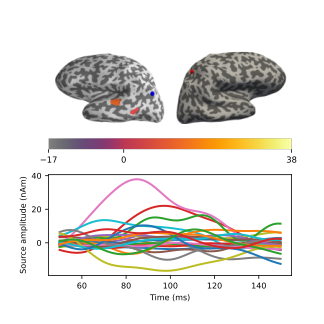
\includegraphics[scale=0.6]{blobs/blob-right_auditory-adaptive-cv}
        \caption{Reweighted - Held-out MSE}
    \end{subfigure}
    \begin{subfigure}{6cm}
        \centering 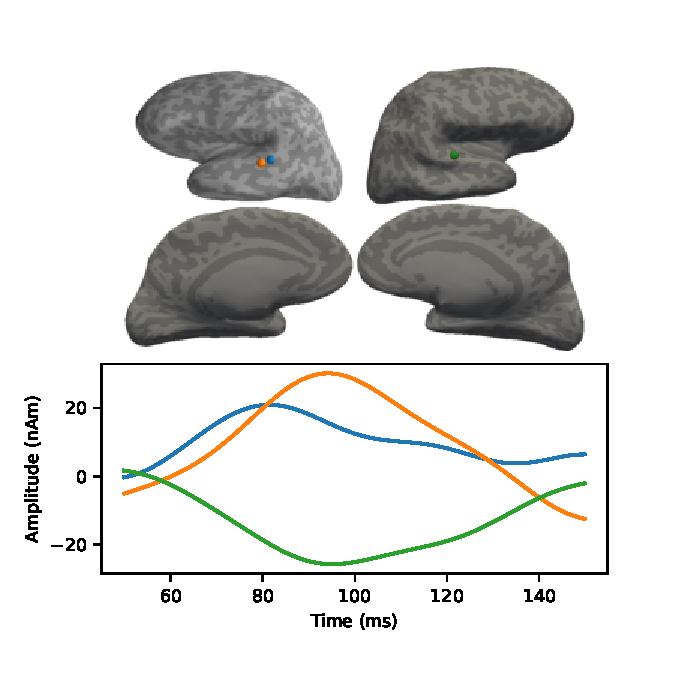
\includegraphics[scale=0.6]{blobs/blob-right_auditory-adaptive-sure}
        \caption{Reweighted - SURE}
    \end{subfigure}
\end{figure}


\subsection{Left visual experiments}

\begin{figure}
    \centering
    \begin{subfigure}{6cm}
        \centering 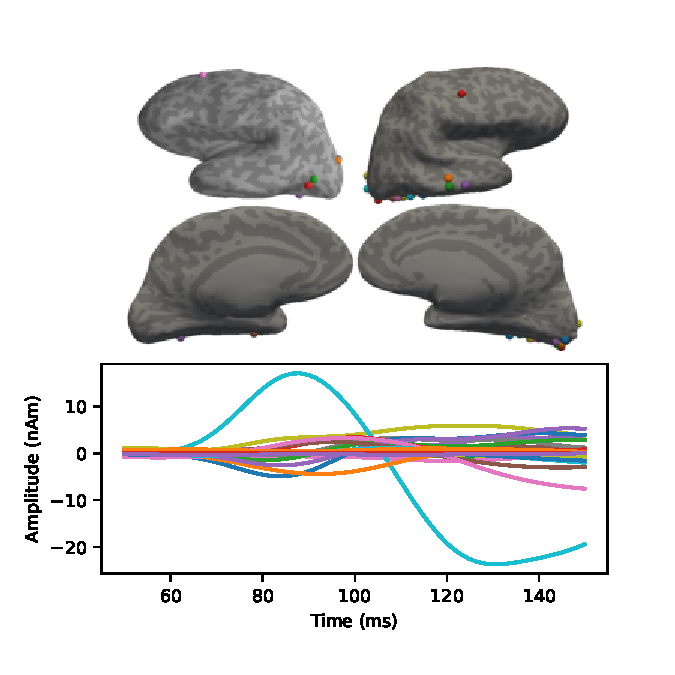
\includegraphics[scale=0.6]{blobs/blob-left_visual-lasso-cv}
        \caption{Lasso - Held-out MSE}
    \end{subfigure}
    \begin{subfigure}{6cm}
        \centering 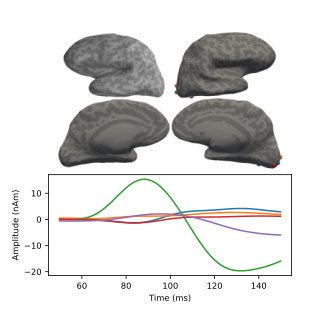
\includegraphics[scale=0.6]{blobs/blob-left_visual-lasso-sure}
        \caption{Lasso - SURE}
    \end{subfigure}

    \begin{subfigure}{6cm}
        \centering 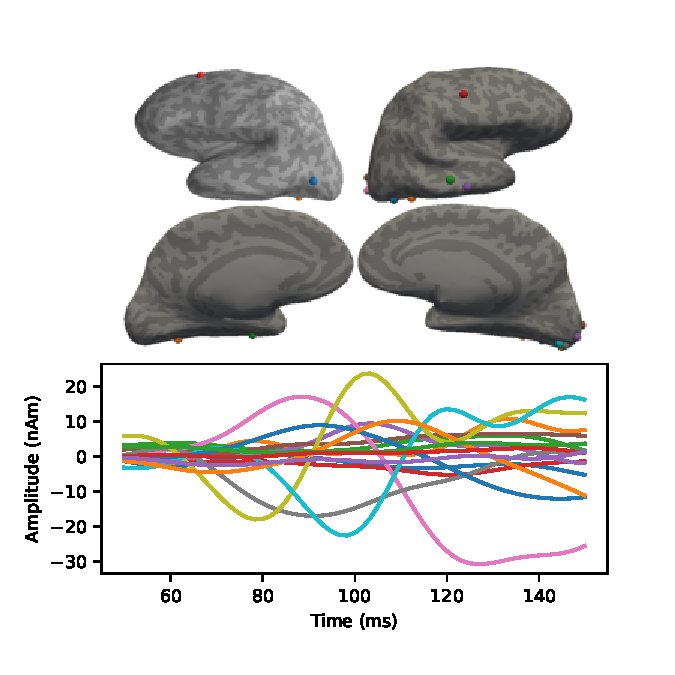
\includegraphics[scale=0.6]{blobs/blob-left_visual-adaptive-cv}
        \caption{Reweighted - Held-out MSE}
    \end{subfigure}
    \begin{subfigure}{6cm}
        \centering 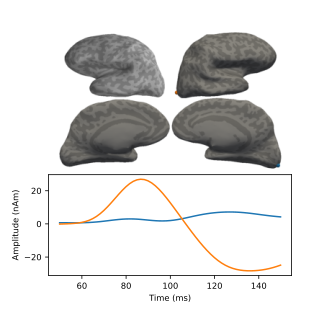
\includegraphics[scale=0.6]{blobs/blob-left_visual-adaptive-sure}
        \caption{Reweighted - SURE}
    \end{subfigure}
\end{figure}


\subsection{Right visual experiments}

\begin{figure}
    \centering
    \begin{subfigure}{6cm}
        \centering 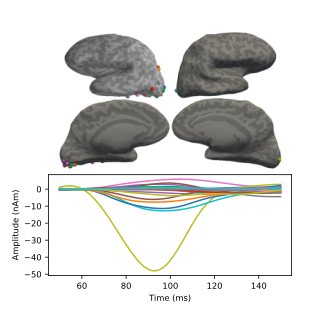
\includegraphics[scale=0.6]{blobs/blob-right_visual-lasso-cv}
        \caption{Lasso - Held-out MSE}
    \end{subfigure}
    \begin{subfigure}{6cm}
        \centering 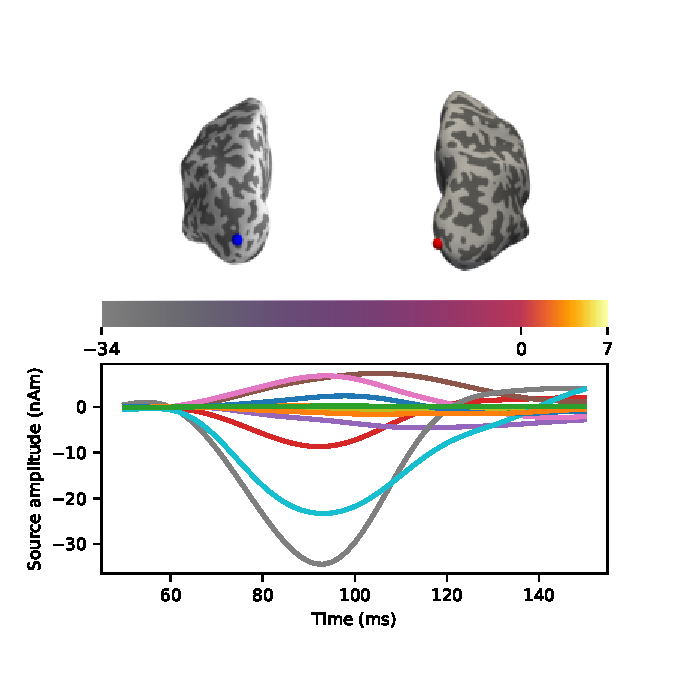
\includegraphics[scale=0.6]{blobs/blob-right_visual-lasso-sure}
        \caption{Lasso - SURE}
    \end{subfigure}

    \begin{subfigure}{6cm}
        \centering 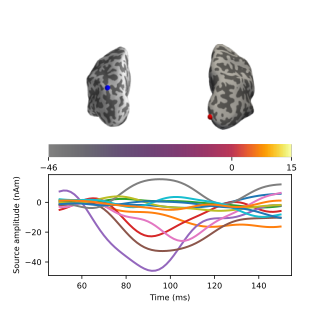
\includegraphics[scale=0.6]{blobs/blob-right_visual-adaptive-cv}
        \caption{Reweighted - Held-out MSE}
    \end{subfigure}
    \begin{subfigure}{6cm}
        \centering 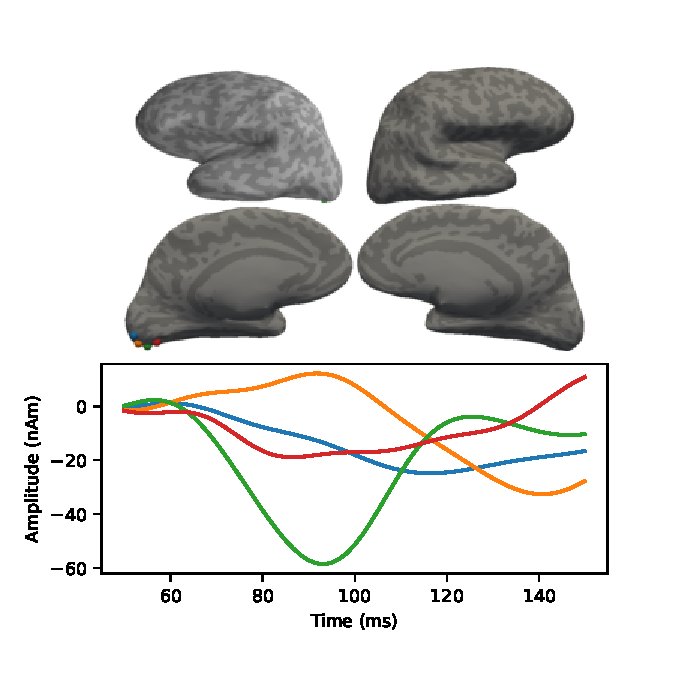
\includegraphics[scale=0.6]{blobs/blob-right_visual-adaptive-sure}
        \caption{Reweighted - SURE}
    \end{subfigure}
\end{figure}


